\section{Zielsetzung}
In diesem Versuch soll die Compton-Wellenlänge $\lambda_\text{C}$ eines Elektrons mithilfe von Röntgenstrahlen bestimmt werden.

\section{Theorie}
\label{sec:Theorie}
\subsection{Der Compton-Effekt}
Ein Photon, das sich an einem Elektron streut und danach eine verlängerte Wellenlänge aufweist, beschreibt den Compton-Effekt.
Bei diesem inelastischen Stoß überträgt das Photon Energie an das Elektron und wird um den Winkel $\theta$ abgelenkt.
Hierdurch wird die Wellenlänge des Photons verlängert.
Die Differenz $\increment \lambda$ der einfallenden und der Compton Wellenlänge kann durch Energie- und Impulserhaltung ausgedrückt werden.
Es gilt:
\begin{equation}\label{eqn:diff_lambda}
    \increment \lambda = \frac{\symup{h}}{\symup{m}_\text{e} \cdot \symup{c}} \cdot (1 - \cos\theta) \, .
\end{equation}
Der Bruch $\frac{\symup{h}}{\symup{m}_\text{e} \cdot \symup{c}}$ ist eine konstante Länge, die sogenannte Compton-Wellenlänge eines Elektrons.
An \eqref{eqn:BraggBedingung} wird ersichtlich, dass bei $\theta = 0°$ die Diffenrenz $\increment \lambda = 0$ und somit minimal ist.
Bei $\theta = 180°$ ist sie maximal, $\increment \lambda = 2 \cdot \lambda_\text{C}$ .
Dieser Vorgang wird durch \autoref{fig:Compton_Effekt} anschaulich dargestellt.

\begin{figure}
    \centering
    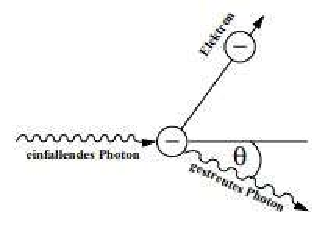
\includegraphics[width=0.4\textwidth]{bilder/compton_effekt.pdf}
    \caption{Schematische Darstellung des Compton-Effekts.\cite{anleitung}}
    \label{fig:Compton_Effekt}
\end{figure}

\subsection{Erzeugung von Röntgenstrahlung}
\noindent
Die für den Versuch benötigten Röntgenstrahlen werden mithilfe einer evakuierten Röhre aus einer Glühkathode erzeugt.
In dieser werden  Elektronen emittiert und auf eine Anode hin beschleunigt.
Die Röntgenstrahlung ensteht bei Auftreffen der Elektronen auf die Anode und setzt sich aus dem kontinuierlichem Bremsspektrum sowie der charakteristischen Röntgenstrahlung des Anodenmaterials zusammen.
Das Bremsspektrum resultiert aus der Abbremsung eines Elektrons im Coulombfeld des Atoms.
Ein Photon bzw. Röntgenquant wird durch dieses Abbremsen emittiert.
Da seine Energie genau dem Energieverlust des abgebremsten Elektrons entspricht und das Elektron entweder einen Teil oder auch seine ganze kinetische Energie abgeben kann, entsteht das sogenannte kontinuierliche Bremsspektrum.

\noindent
Das Anodenmaterial wird so ionisiert.
Ein Elektron aus einer äußeren Schale kann nach Emittieren eines Photons in eine Innere fallen.
Hierbei hat das Photon genau die Energiedifferenz der beiden Energieniveaus, somit entsteht kein kontinuierliches sondern ein Spektrum aus scharfen Linien.
Dieses sogenannte charakteristische Spektrum hängt vom Anodenmaterial der Röntgenröhre ab.


\subsection{Transmission und Absorption bei Aluminium}
Mithilfe der Absorption und Transmission von Röntgenstrahlung durch Aluminium kann die Compton-Wellenlänge bestimmt werden.
Diese sind von der Wellenlänge abhängig.
Es besteht ein antiproportionaler Zusammenhang zwischen Transmission und Wellenlänge, bei großer Wellenlänge ist die Transmission klein.
Somit ist die Transmission bei der Compton verschobenen Wellenlänge kleiner als bei der einfallenden.
Für die Absorption der Photonen in einer Materie der Dicke $d$ gilt für die Intensität $I$ das Delamber'sche Gesetz:
\begin{equation*}
    I = I_0 \cdot e^{-\mu d} \, ,
\end{equation*}
wobei $I_0$ die einfallende Intensität und $\mu$ den Absorptionskoeffizienten beschreibt.
Dieser Absorbtionskoeffizient setzt sich durch Addition der Absorbtionskoeffizienten für Paarbildung $\mu_\text{Paar}$, Photoeffekt $\mu_\text{Photo}$ und Comptoneffekt $\mu_\text{Com}$ zusammen.

\subsection{Bragg Bedingung}
Mithilfe der Bragg'schen Reflexion kann die Energie $E$ und somit die Wellenlänge $\lambda$ der Röntgenstrahlung bestimmt werden.
Hierbei fällt Röntgenlicht auf ein dreidimensionales Gitter.
Jedes Gitteratom sorgt für eine Beugung der Photonen.
Dadurch interferieren die Strahlen miteinander.
Konstruktive Interferenz passiert beim sogenannten Glanzwinkel $\alpha$.
Ist die Gitterkonstante $d$ bekannt, kann mit der Bragg'schen Bedingung, siehe \eqref{eqn:BraggBedingung},
die Wellenlänge $\lambda$ der Röntgenstrahlung und somit die Energie $E$ bestimmt werden.

\begin{equation}
    \label{eqn:BraggBedingung}
    2 \cdot d \cdot \sin\alpha = n \cdot \lambda
\end{equation}